\section{Rilascio}

\subsection{Come eseguire il rilascio su Windows}
Per generare l'eseguibile su Windows è necessario eseguire il file:
\newline{}\centerline{\textbf{win-dist.bat}}\newline{}
Viene generato un virtual environment di Python (se non presente), successivamente dopo aver installato tutte le librerie viene generato l'eseguibile all'interno della cartella \textit{dist} con il nome \textit{SSD.exe}\\
Per leggere gli eventuali messaggi di errore, è necessario rimuovere il flag \textit{--windowed} dal file \textit{win-dist.bat}. Una volta lanciato il programma comparirà una finestra del terminale dove poter leggere gli errori presenti.
\begin{figure}[H]
    \centering
    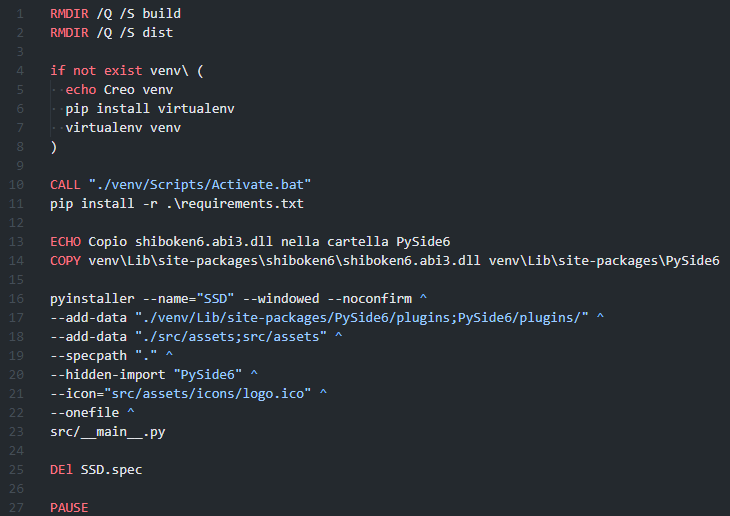
\includegraphics[scale = 0.6]{components/img/pyinstaller.png}
    \caption{File win-dist.bat}
    \label{fig:File win-dist.bat}
\end{figure}
